% ================================================================
%  Generative Augmentation for Data-Constrained MTSF
%  Compile: pdfLaTeX -> BibTeX -> pdfLaTeX -> pdfLaTeX
%  Overleaf: compiler = pdfLaTeX, bibliography = BibTeX
% ================================================================
\documentclass[aspectratio=169,10pt]{beamer}

% ---------- THEME ----------
\usetheme{Boadilla}
\usecolortheme{whale}
\setbeamertemplate{navigation symbols}{}
\setbeamertemplate{footline}{%
  \leavevmode%
  \hbox{%
    \begin{beamercolorbox}[wd=.65\paperwidth,ht=2.25ex,dp=1ex,leftskip=.3cm]%
        {author in head/foot}%
      \usebeamerfont{author in head/foot}%
      \insertshortauthor\quad|\quad\insertshorttitle
    \end{beamercolorbox}%
    \begin{beamercolorbox}[wd=.35\paperwidth,ht=2.25ex,dp=1ex,rightskip=.3cm,right]%
        {date in head/foot}%
      \usebeamerfont{date in head/foot}%
      \insertshortdate{}\quad
      \insertframenumber{} / \inserttotalframenumber
    \end{beamercolorbox}}%
  \vskip0pt}

% ---------- PACKAGES ----------
\usepackage{amsmath,amssymb,mathtools}
\usepackage{graphicx}
\usepackage{booktabs}
\usepackage{array}
\usepackage{xcolor}
\usepackage{colortbl}
\usepackage{tikz}
\usetikzlibrary{arrows.meta,positioning}
\usepackage{pgfplots}
\pgfplotsset{compat=1.18}
\usepackage[round]{natbib}   % round = parentheses for author-year

% ---------- COLORS ----------
\definecolor{myblue}{RGB}{31,119,180}
\definecolor{myred}{RGB}{180,30,30}
\definecolor{mygreen}{RGB}{30,130,30}
\definecolor{mygray}{RGB}{110,110,110}
\definecolor{boxblue}{RGB}{210,228,252}
\definecolor{boxyellow}{RGB}{255,250,200}
\definecolor{boxgreen}{RGB}{210,245,210}

% ---------- TITLE ----------
\title[Generative Data Augmentation for Time Series Forecasting]{%
  Generative Data Augmentation for\\
 Time Series Forecasting}
\subtitle{A Spectral Preserving Baseline Study}
\author[Jinyu Li]{Jinyu Li}
\institute[Your Lab]{University College London}
\date[Apr 2026]{April 20, 2026}

% ================================================================
\begin{document}
% ================================================================

\begin{frame}
  \titlepage
\end{frame}

\begin{frame}{Outline}
  \tableofcontents
\end{frame}

% ================================================================
\section{Motivation}
% ================================================================

\begin{frame}{Motivation: Time Series Forecasting Models Training Limitations}
  \begin{columns}[T]
    \column{0.50\textwidth}
      \textbf{Input Variables}
      \begin{itemize}
        \item $\mathbf{X}\!\in\!\mathbb{R}^{T\times C}$: Weather data set includes $C$ features contains $T$ time steps in total.
        \item $\mathbf{X}_{t-L+1 : t}\!\in\!\mathbb{R}^{L \times C }$: Weather data includes $C$ features from time step $t-L+1$ to $t$. 
      \end{itemize}
      \textbf{Prediction Target}
      \begin{itemize}
        \item $y_{t+d}\!\in\!\mathbb{R}$: Weather data of 'temperature at $850 hpa(Kelvin)$' on time step $t+d$.
      \end{itemize}
      \textbf{Target Function $f(\cdot)$}
      \begin{itemize}
        \[
        f1:\mathbf{X}_{t-L+1 : t}  \rightarrow\ y_{t+d}
        \]
      \end{itemize}
      

\column{0.50\textwidth}
  \textbf{Limitations}
  \begin{itemize}
        \item Forecasting models process each sample $(\mathbf{X}_{t-L+1 : t}, y_{t+d})$ as a fixed pair in a left to right order in every epoch.
        \item Similar to the limitation in autoregressive language models with fixed factorization [cite 2507.15857].
        \item $\mathbf{x_t} \in \mathbb{R}^{C}$: the observation vector at time step $t$, including  $C$ features.
        \item $\mathbf{x_1}, \mathbf{x_2}, \ldots, \mathbf{x_n}$: a consecutive sequence.
        \item $p(\mathbf{x_1}, \mathbf{x_2}, \ldots, \mathbf{x_n}) = p(\mathbf{x_1})\cdot p(\mathbf{x_1} \mid \mathbf{x_2}) \cdot p(\mathbf{x_3} \mid \mathbf{x_1},\mathbf{x_2})\cdot \ldots \cdot p(\mathbf{x_n} \mid \mathbf{x_1}, \mathbf{x_2}, \ldots, \mathbf{x_{n-1}})$
        \item The conditional probability of the current observation given all preceding time steps reflects the left to right fixed factorization of the joint distribution.

      \end{itemize}
  \vspace{0.5em}

  \end{columns}
\end{frame}

\begin{frame}{Motivation: Early Converge or Well Trained}
  \begin{columns}[T]
    \column{0.50\textwidth}
      \textbf{A Common Objection}
      \begin{itemize}{}
        \item Task specific Time Series forecasting models already learn the training data
        thoroughly. Synthetic data cannot help them.
      \end{itemize}

\column{0.50\textwidth}
  \textbf{Why the Objection May Be Wrong}
  \begin{itemize}
    \item \textbf{Convergence $\neq$ Thorough Learning}\\
          Models may early converge on frequent patterns,
          missing rare events and tail samples.
    \item \textbf{Same Distribution but Diverse Samples}
          Expose the model to diverse temporal dependencies
                  and tail samples unseen in real data $\mathbf{X}$, improving generalisation ability.
  \end{itemize}
  \vspace{0.5em}
  \begin{block}{Research Question}
    \centering
    Can Synthetic data improve forecasting performance?
  \end{block}

  \end{columns}
\end{frame}

% ================================================================
\section{Literature Review}
% 需要优化数学表述（diffusion怎么做数据预测的？把diverse的data exposure表现出来.diffusion和AR有啥区别）
% 
% ================================================================

% ================================================================
% Slide 1 / 2
% ================================================================
\begin{frame}{Literature: Diffusion and AR — Objectives (1/2)}
  \begin{block}{Key Reference}
    \citet{prabhudesai2025diffusion}:
    \emph{Diffusion Beats Autoregressive in Data-Constrained Settings.}
    arXiv:2507.15857
  \end{block}
  \vspace{0.4em}

  \textbf{Shared Setup.}\;
  Let $\mathbf{x} = (x_1,\ldots,x_L)\in\mathcal{V}^L$ be a training sequence
  of length $L$ from vocabulary $\mathcal{V}$.

  \vspace{0.5em}
  \textbf{Autoregressive (AR) — fixed left-to-right factorisation:}
  \[
    \mathcal{L}_{\mathrm{AR}}
      = -\sum_{j=1}^{L}\log p_\theta\!\left(x_j \mid \mathbf{x_{<j}}\right)
  \]

  \begin{itemize}
    \item $x_j\in\mathcal{V}$: token at position $j$ (prediction target)
    \item $\mathbf{x_{<j}}=(x_1,\ldots,x_{j-1})$: all preceding tokens,
          enforced by a \emph{causal attention mask}
    \item Each sequence is one set of prediction
          tasks per epoch (left $\to$ right, same order)
    \item Fixed factorisation and zero diversity across epochs
  \end{itemize}
\end{frame}

% ================================================================
% Slide 2 / 2
% ================================================================
\begin{frame}{Literature: Diffusion and AR — Objectives (2/2)}
  \textbf{Masked Diffusion — randomised masking (bidirectional attention):}
  \[
    \mathcal{L}_{\mathrm{Diff}}
      = -\;\mathbb{E}_{r,\,\tilde{x}\sim q_{r}}\!
        \left[\,\frac{1}{r}
          \sum_{i\in\mathcal{M}}
            \log p_\theta\!\left(x_i \mid \tilde{x}\right)
        \right]
  \]

  \begin{itemize}
    \item $r\sim\mathcal{U}(0,1)$: mask ratio, re-sampled \emph{every} training step
    \item $\mathbf{\tilde{x}}$: corrupted sequence — each token replaced by
          mask independently with probability $r$
    \item $\mathcal{M}=\{i:\tilde{x}_i=MASK\}$:
          set of masked positions, changes every step
    \item $x_i$: original token at masked position $i$ (prediction target)
    \item $\tfrac{1}{r}$: importance weight; loss is compute by ELBO on
          $\log p(x)$
    \item $2^{L}$ distinct masking patterns per sequence, leading to implicit data augmentation.
  \end{itemize}
\end{frame}

\begin{frame}{Literature: Quickly Saturate or Late Overfitting}
\begin{columns}[T]
    \column{0.50\textwidth}
      \begin{block}{Empirical Evidence (Table 1)}
        \small
        C4 (Colossal Clean Crawled Corpus), limited data.\\[0.2em]
        Each point represents a model trained until convergence.\\[0.2em]
        Effective data half-life $R^{*}_{D}$:\\[0.2em]
        \quad Diffusion:\; $R^{*}_{D}\approx 500$ epochs\\
        \quad AR:\hspace{2.6em} $R^{*}_{D}\approx 15$\phantom{0} epochs
      \end{block}

    \column{0.50\textwidth}
      \begin{alertblock}{Take-Away for Time Series}
        \small
        Advantage could be data-exposure diversity,
        except for architecture.\\[0.2em]
        Can we introduce the diversity via synthetic data?
      \end{alertblock}
  \end{columns}
\end{frame}

% ================================================================
\section{Why Not Use Generative Models Directly?}
% 查询确认chronos2是generative模型吗？
% 表明目前generative 模型就是干不过AR模型？
% independently improved是个好事情
% ================================================================

\begin{frame}{Why Not Use Generative Models Directly for Forecasting?}
  \begin{columns}[T]
    \column{0.50\textwidth}

      \textbf{Arg.\ 1 — Task-specific models still dominate}
      \begin{itemize}
        \item CrossFormer, DeformTime, Sonnet: well designed
             models with task specific HPO.
        \item On domain specific benchmarks, they
              consistently outperform generic generative
              models, with far fewer parameters.
      \end{itemize}

      \vspace{0.6em}
      \textbf{Arg.\ 2 — Generative models require lots of data}
      \begin{itemize}
        \item Chronos \citep{ansari2024chronos}: autoregressive
              generative model; requires $>$84B training observations
              for competitive zero-shot performance
      \end{itemize}

    \column{0.50\textwidth}

      \textbf{Arg.\ 3 — Generation is an easier task than forecasting}
      \vspace{0.3em}

      \begin{tabular}{@{}ll@{}}
        Generation:   & learn $p(\mathbf{X})$ \\[4pt]
        Forecasting:  & learn $p(\mathbf{X}_{t+1:t+H}\mid\mathbf{X}_{t-L+1:t})$
      \end{tabular}

      \vspace{0.4em}
      \begin{itemize}
        \item Generating capturing marginal distribution.
        \item Forecasting requires precise conditional accuracy
              under limited data.
      \end{itemize}

      \vspace{0.3em}
      \begin{alertblock}{Strategy: decouple the two tasks}
        \small
        \textbf{Generator}:\\
        distribution-preserving synthetic data\\[0.4em]
        \textbf{Forecaster} (CrossFormer / DeformTime / Sonnet):\\
        trained on real $+$ synthetic\\[0.4em]
     Two components independently improvable
      \end{alertblock}
  \end{columns}
\end{frame}

% ================================================================
\section{Research Hypothesis}
% step1 any 这个肯定不对。直接移出去，不好解释
% 不如用iaaft来解释
% 更好的数学表示来表征学习过程（以及性质。）（不要用笼统的语言）
% ================================================================

\begin{frame}{Research Hypothesis: A Controlled First Step}
  \begin{columns}[T]
    \column{0.54\textwidth}
      \textbf{Stepwise Validation Strategy}
      \vspace{0.4em}

      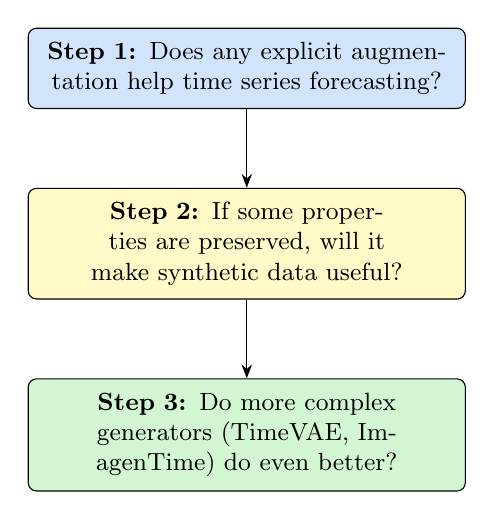
\begin{tikzpicture}[
          node distance=1.0cm,
          box/.style={draw, rounded corners=3pt,
                      text width=5.2cm, align=center,
                      font=\small, inner sep=5pt}]
        \node[box, fill=boxblue] (s1) {%
          \textbf{Step 1:} Does any explicit augmentation
          help time series forecasting?};
        \node[box, fill=boxyellow, below=of s1] (s2) {%
          \textbf{Step 2:} If some properties are preserved, will
          it make synthetic data useful?};
        \node[box, fill=boxgreen, below=of s2] (s3) {%
          \textbf{Step 3:} Do more complex generators
          (TimeVAE, ImagenTime) do even better?};
        \draw[-{Stealth[length=5pt]}] (s1) -- (s2);
        \draw[-{Stealth[length=5pt]}] (s2) -- (s3);
      \end{tikzpicture}

    \column{0.46\textwidth}
      \textbf{Start with IAAFT-MV?}
      \begin{itemize}
        \item Non-parametric, \textbf{fully controllable}: preserved
              and randomized properties are known
        \item Acts as an interpretable baseline.
        \item modern complex generators should have even
              greater potential
        \item If it fails, we learn what property
              matters (power spectrum is not enough)
      \end{itemize}
      \vspace{0.4em}
      \begin{alertblock}{Falsifiable Claim}
        \small
        Surrogates with same power spectrum (raw $+$ synthetic) will
        not significantly degrade, and in some settings will
        improve forecasting performance.
      \end{alertblock}
  \end{columns}
\end{frame}

% ================================================================
\section{Method}
% ================================================================
% ================================================================
% Slide 1 / 2: 频谱分解与目标
% ================================================================
\begin{frame}{Method: IAAFT-MV --- Spectral Decomposition \& Goal}

  \textbf{Notation.}\;
  $\mathbf{X}\!\in\!\mathbb{R}^{T\times C}$: original multivariate series;
  channel $k$: $\mathbf{x}_k\!\in\!\mathbb{R}^{T}$,\;
  $x_{k,t}\in\mathbb{R}$ the value at time $t$.

  \vspace{0.4em}
  \textbf{DFT of channel $k$} \quad ($f = 0, 1, \ldots, T{-}1$):
  \[
    X_k(f)
      \;=\; \mathcal{F}\{\mathbf{x}_k\}(f)
      \;=\; \sum_{t=0}^{T-1} x_{k,t}\, e^{-i 2\pi f t / T}
      \;\in\; \mathbb{C}
  \]

  Written in polar form:
  \[
    X_k(f)
      = \underbrace{A_k(f)}_{\displaystyle |X_k(f)|\;\in\;\mathbb{R}_{\ge 0}}
        \cdot\;
        e^{\,i\;\underbrace{\phi_k(f)}_{\displaystyle \arg X_k(f)\;\in\;[-\pi,\pi)}}
  \]

  \vspace{0.3em}
  \begin{columns}[T]
    \column{0.52\textwidth}
      \begin{tabular}{@{}lll@{}}
        \toprule
        Quantity & Symbol & Encodes \\
        \midrule
        Amplitude spectrum & $A_k(f)$ & signal strength at freq.\ $f$ \\
        Power spectrum     & $A_k(f)^2$ & autocorrelation structure$^{*}$ \\
        Phase spectrum     & $\phi_k(f)$ & temporal arrangement \\
        \bottomrule
      \end{tabular}

      \vspace{0.2em}
      {\footnotesize $^{*}$via Wiener--Khinchin:
        $R_{kk}(\tau)\;\xleftrightarrow{\;\mathcal{F}\;}\;A_k(f)^2$}

    \column{0.48\textwidth}
      \textbf{Goal}: generate surrogate $\tilde{\mathbf{X}}$
      \vspace{0.2em}

      \begin{tabular}{@{}p{3.6cm}c@{}}
        \toprule
        Property & Preserved? \\
        \midrule
        Amplitude dist.\ $p(\mathbf{x}_k)$      & \checkmark \\
        Power spectrum $A_k(f)^2$                & \checkmark \\
        Cross-channel phase gap                  & \checkmark \\
        \midrule
        Absolute phase $\phi_k(f)$               & $\times$\;randomized \\
        \bottomrule
      \end{tabular}
  \end{columns}
\end{frame}

% ================================================================
% Slide 2 / 2: 算法
% ================================================================
\begin{frame}{Method: IAAFT-MV --- Algorithm}
  \begin{columns}[T]
    \column{0.52\textwidth}

      \textbf{Step 1 — Shared random phase shift}\\[0.2em]
      Draw \emph{one} random offset per frequency, shared across
      all $C$ channels:
      \[
        \Delta\phi(f)
          \;\overset{\mathrm{i.i.d.}}{\sim}\;
          \mathcal{U}(-\pi,\,\pi),
        \quad f=0,\ldots, T/2
      \]
      Apply simultaneously to every channel:
      \[
        
          X_k^{(0)}(f)
            = A_k(f)\;
              e^{\,i\bigl(\phi_k(f)\,+\,\Delta\phi(f)\bigr)
        }
      \]
      $\Rightarrow\;\phi_k(f)-\phi_j(f)$ unchanged
      (cross-channel)

      \vspace{0.4em}
      \textbf{Step 2 — IDFT}
      \[
        \mathbf{x}_k^{(0)}
          = \mathcal{F}^{-1}\!\left\{X_k^{(0)}\right\}
          \in \mathbb{R}^{T}
      \]

    \column{0.48\textwidth}

      \textbf{Steps 3--4 — Iterative correction}
      (repeat until rank order converges)

      \medskip
      \textit{(a) Spectral step}: replace amplitudes with original,
      keep current phase:
      \[
        \tilde{X}_k^{(n)}(f)
          = A_k(f)\cdot
            e^{\,i\,\arg X_k^{(n)}(f)},
        \;\;
        \tilde{\mathbf{x}}_k^{(n)}
          = \mathcal{F}^{-1}\!\left\{\tilde{X}_k^{(n)}\right\}
      \]

      \textit{(b) Amplitude step}: rank-reorder to match
      original values:
      \[
        x_{k,t}^{(n+1)}
          = \mathbf{x}_k^{\mathrm{sorted}}\!
            \left[\,\mathrm{rank}(\tilde{x}_{k,t}^{(n)})\,\right]
      \]

      \begin{alertblock}{Result}
        \small
        Fixed point $\tilde{\mathbf{X}}$ satisfies
        $p(\tilde{\mathbf{x}}_k)=p(\mathbf{x}_k)$ and
        $|\tilde{X}_k(f)|=A_k(f)$,\\
        but with randomized temporal phase
        $\;\Rightarrow\;$
        \textbf{diversity without distribution shift}
      \end{alertblock}
  \end{columns}
\end{frame}

% ================================================================
\section{Visualization}
% ================================================================

\begin{frame}{Synthetic Data Quality: Time Domain \& Frequency Domain}
%%这个summary 说的没头没尾的
  \begin{columns}[T]
    \column{0.50\textwidth}
      \textbf{Time Domain (raw vs.\ surrogate)}
      \vspace{0.3em}

      % Uncomment after uploading figure:
      % \includegraphics[width=\linewidth]{figures/MV-TIME-03-13.pdf}
      \begin{center}
        \fbox{\parbox{0.9\linewidth}{%
          \centering\vspace{1.3cm}
          {\small\texttt{[Insert MV-TIME-03-13.pdf]}}\\[0.2em]
          {\footnotesize raw vs.\ surrogate per channel}
          \vspace{1.3cm}}}
      \end{center}
      {\small Waveforms differ; amplitude distribution consistent.}

    \column{0.50\textwidth}
      \textbf{Power Spectrum (raw vs.\ surrogate)}
      \vspace{0.3em}

      % Uncomment after uploading figure:
      % \includegraphics[width=\linewidth]{figures/MV-FREQ-03-13.pdf}
      \begin{center}
        \fbox{\parbox{0.9\linewidth}{%
          \centering\vspace{1.3cm}
          {\small\texttt{[Insert MV-FREQ-03-13.pdf]}}\\[0.2em]
          {\footnotesize overlay: raw vs.\ surrogate spectra;\\
           annotate $\Delta\phi$ shifts with arrows}
          \vspace{1.3cm}}}
      \end{center}
      {\small Spectra overlap per channel; intra-channel phases randomized.}
  \end{columns}
  \vspace{0.3em}
  \begin{block}{Summary}
    IAAFT-MV surrogates are \textbf{statistically faithful but
    informationally distinct}: each is a valid new realization of
    the same spectral process.
  \end{block}
\end{frame}

% ================================================================
\section{Experiments}
% ================================================================

\begin{frame}{Experimental Setup}
%%要调整  简洁就好， 内容太多
  \begin{columns}[T]
    \column{0.50\textwidth}
      \textbf{Dataset: WeatherBench}
      \begin{itemize}
        \item 3 cities: Cape Town (CT), Hong Kong (HK), London (LN)
        \item 5 variables: temperature, humidity, wind ($u,v$), pressure
        \item Full span: 1979--2019 (40 years, daily)
        \item \textbf{Training source}: 2003--2013 (10 years)
        \item \textbf{Augmentation}: $1\times$ IAAFT-MV surrogate
              of training source
        \item \textbf{Test}: years 2016, 2017, 2018 (held-out)
      \end{itemize}

    \column{0.50\textwidth}
      \textbf{Models \& Evaluation}
      \begin{itemize}
        \item \textbf{AR forecasting models}:
          \begin{itemize}
            \item CrossFormer (cross-time Transformer)
            \item DeformTime (deformable attention)
            \item Sonnet (in-house AR model)
          \end{itemize}
        \item Horizon $H=28$ d, input window $L=56$ d
        \item HPO: Bayesian optimization per model $\times$ city
        \item \textbf{Metrics} (avg.\ over 2016/17/18):
          \begin{itemize}
            \item Pearson $r$ ($\uparrow$)
            \item MAE ($\downarrow$)
            \item sMAPE ($\downarrow$)
          \end{itemize}
      \end{itemize}
  \end{columns}
\end{frame}

% ------- TABLE 1 -------
\begin{frame}{Results --- Table 1: AR Models on Raw Data Only}
% 这里换成规范的制图
  \vspace{-0.2em}
  \begin{center}
    {\small\textit{$H=28$ days; metrics averaged over test years 2016/2017/2018}}
  \end{center}
  \vspace{0.1em}
  \begin{table}
    \centering
    \footnotesize
    \setlength{\tabcolsep}{6pt}
    \begin{tabular}{l rrr rrr rrr}
      \toprule
      & \multicolumn{3}{c}{\textbf{Cape Town}}
      & \multicolumn{3}{c}{\textbf{Hong Kong}}
      & \multicolumn{3}{c}{\textbf{London}} \\
      \cmidrule(lr){2-4}\cmidrule(lr){5-7}\cmidrule(lr){8-10}
      \textbf{Model}
        & $r{\uparrow}$ & MAE${\downarrow}$ & sMAPE${\downarrow}$
        & $r{\uparrow}$ & MAE${\downarrow}$ & sMAPE${\downarrow}$
        & $r{\uparrow}$ & MAE${\downarrow}$ & sMAPE${\downarrow}$ \\
      \midrule
      CrossFormer
        & 0.442 & 3.840 & 21.89
        & 0.751 & 1.500 &  9.26
        & 0.681 & 3.320 & 26.26 \\
      DeformTime
        & 0.454 & 3.815 & 21.77
        & 0.753 & 1.535 &  9.46
        & 0.669 & 3.367 & 26.41 \\
      Sonnet
        & 0.466 & 3.790 & 21.64
        & 0.762 & 1.521 &  9.40
        & 0.678 & 3.331 & 26.27 \\
      \bottomrule
    \end{tabular}
  \end{table}
  \vspace{0.2em}
  {\footnotesize Training: 2003--2013 raw only;\;
   best HPO config per city $\times$ model;\; seed\,$=42$.}
\end{frame}

% ------- TABLE 2 -------
\begin{frame}{Results --- Table 2: Raw $+$ IAAFT-MV Synthetic}
  \vspace{-0.2em}
  \begin{center}
    {\small\textit{Same setup; training augmented with
    $1\times$ IAAFT-MV surrogate of 2003--2013}}
  \end{center}
  \vspace{0.1em}
  \begin{table}
    \centering
    \footnotesize
    \setlength{\tabcolsep}{5pt}
    \begin{tabular}{l rrr rrr rrr}
      \toprule
      & \multicolumn{3}{c}{\textbf{Cape Town}}
      & \multicolumn{3}{c}{\textbf{Hong Kong}}
      & \multicolumn{3}{c}{\textbf{London}} \\
      \cmidrule(lr){2-4}\cmidrule(lr){5-7}\cmidrule(lr){8-10}
      \textbf{Model}
        & $r{\uparrow}$ & MAE${\downarrow}$ & sMAPE${\downarrow}$
        & $r{\uparrow}$ & MAE${\downarrow}$ & sMAPE${\downarrow}$
        & $r{\uparrow}$ & MAE${\downarrow}$ & sMAPE${\downarrow}$ \\
      \midrule
      CrossFormer
        & \textcolor{mygreen}{\textbf{0.461}}
        & \textcolor{mygreen}{\textbf{3.793}}
        & \textcolor{mygreen}{\textbf{21.63}}
        & \textcolor{mygray}{0.750}
        & \textcolor{myred}{1.540}
        & \textcolor{myred}{9.54}
        & \textcolor{mygray}{0.674}
        & \textcolor{mygray}{3.333}
        & \textcolor{mygray}{26.27} \\[1pt]
      DeformTime
        & \textcolor{mygray}{0.454}
        & \textcolor{mygray}{3.809}
        & \textcolor{mygray}{21.73}
        & \textcolor{mygreen}{\textbf{0.760}}
        & \textcolor{mygreen}{\textbf{1.511}}
        & \textcolor{mygreen}{\textbf{9.30}}
        & \textcolor{mygreen}{\textbf{0.686}}
        & \textcolor{mygreen}{\textbf{3.275}}
        & \textcolor{mygreen}{\textbf{25.82}} \\[1pt]
      Sonnet
        & \textcolor{myred}{0.459}
        & \textcolor{mygray}{3.808}
        & \textcolor{mygray}{21.75}
        & \textcolor{myred}{0.753}
        & \textcolor{mygreen}{\textbf{1.512}}
        & \textcolor{mygray}{9.39}
        & \textcolor{myred}{0.668}
        & \textcolor{myred}{3.386}
        & \textcolor{myred}{26.71} \\
      \bottomrule
    \end{tabular}
  \end{table}
  {\footnotesize
   \textcolor{mygreen}{\textbf{Green}}: improved;\;
   \textcolor{mygray}{Gray}: $|\Delta|<1\%$ neutral;\;
   \textcolor{myred}{Red}: degraded.}
  \vspace{0.2em}
  \begin{block}{Observations}
    \small
    (1)~\textbf{DeformTime}: clear improvement on HK
        ($r$: $0.753\!\to\!0.760$; MAE: $1.535\!\to\!1.511$) and
        London ($r$: $0.669\!\to\!0.686$; MAE: $3.367\!\to\!3.275$).
    \;(2)~\textbf{CrossFormer}: improvement on Cape Town.
    \;(3)~\textbf{Sonnet}: slight degradation in some settings.
    \;(4)~Is this seed artifact? $\to$ Scaling experiment needed.
  \end{block}
\end{frame}

% ================================================================
\section{Scaling Validation}
% ================================================================

\begin{frame}{Is the Improvement Real? Scaling Synthetic Data Volume}
% 这里考虑优化一下图片和表
  \begin{columns}[T]
    \column{0.44\textwidth}
      \begin{block}{Hypothesis}
        If IAAFT-MV surrogates are genuinely informative, then
        \textbf{more synthetic data} should yield
        \textbf{monotonically better} performance (data scaling law).
      \end{block}
      \vspace{0.5em}

      \textbf{Experiment Design}
      \vspace{0.2em}

      \begin{tabular}{@{}ll@{}}
        \toprule
        \textbf{Group} & \textbf{Training Data} \\
        \midrule
        Baseline  & Raw only (10yr) \\
        Current   & Raw $+$ $1\times$ Syn (10yr) \\
        \midrule
        \textbf{Plan A} & Raw $+$ $1\times$ Syn (20yr) \\
        \textbf{Plan B} & Raw $+$ $2\times$ Syn (10yr) \\
        \bottomrule
      \end{tabular}
      \vspace{0.3em}

      {\small Plan A and B each double the synthetic volume via
       different mechanisms, separating \emph{source-length}
       from \emph{copy-count} effects.}

    \column{0.56\textwidth}
      \textbf{Expected Outcomes (schematic)}
      \vspace{0.2em}

      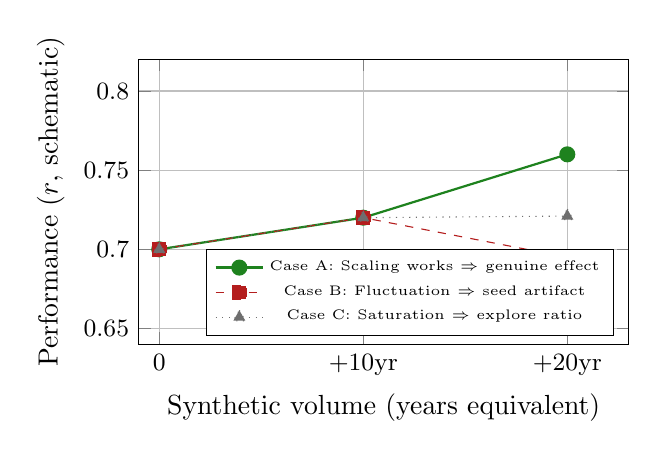
\begin{tikzpicture}
        \begin{axis}[
            width=7.8cm, height=5.2cm,
            xlabel={Synthetic volume (years equivalent)},
            ylabel={Performance ($r$, schematic)},
            xmin=-1, xmax=23,
            xtick={0,10,20},
            xticklabels={0, +10yr, +20yr},
            ymin=0.64, ymax=0.82,
            legend pos=south east,
            legend style={font=\tiny, cells={align=left}},
            grid=major,
            tick label style={font=\small}
          ]
          \addplot[color=mygreen, mark=*, thick, mark size=2.5pt]
            coordinates {(0,0.70)(10,0.72)(20,0.76)};
          \addlegendentry{Case A: Scaling works $\Rightarrow$ genuine effect}
          \addplot[color=myred, mark=square*, dashed, mark size=2.5pt]
            coordinates {(0,0.70)(10,0.72)(20,0.695)};
          \addlegendentry{Case B: Fluctuation $\Rightarrow$ seed artifact}
          \addplot[color=mygray, mark=triangle*, dotted, mark size=2.5pt]
            coordinates {(0,0.70)(10,0.72)(20,0.721)};
          \addlegendentry{Case C: Saturation $\Rightarrow$ explore ratio}
        \end{axis}
      \end{tikzpicture}
  \end{columns}
\end{frame}

% ================================================================
\section{Future Work}
% ================================================================
% 这块timevae真的只关于 time吗？其实不然吧。diffusion也不是只关于T/F
\begin{frame}{Future Work: Towards Deep Generative Surrogates}
  \begin{columns}[T]
    \column{0.44\textwidth}
      \textbf{Current Limitations of IAAFT-MV}
      \begin{itemize}
        \item Non-parametric: cannot learn nonlinear dynamics
        \item Preserves only 2nd-order statistics (power spectrum)
        \item Phase randomization may be too aggressive for strongly
              coherent signals
      \end{itemize}
      \vspace{0.4em}

      \textbf{Planned Methods}
      \begin{block}{TimeVAE}
        \small
        VAE for multivariate TS generation.\\
        $\min\;
         \mathcal{L}_{\mathrm{recon}}
         + \beta\,D_{\mathrm{KL}}(q_\phi\,\|\,p)$\\
        Focus: time-domain statistical fidelity.
      \end{block}
      \vspace{0.3em}
      \begin{block}{ImagenTime}
        \small
        Diffusion-based TS generation.\\
        Iterative denoising $\to$ richer diversity.\\
        Focus: joint time $+$ frequency domain.
      \end{block}

    \column{0.56\textwidth}
      \textbf{Research Roadmap}
      \vspace{0.3em}

      \begin{tabular}{@{}lll@{}}
        \toprule
        \textbf{Method} & \textbf{Type} & \textbf{What it Preserves} \\
        \midrule
        IAAFT-MV   & Non-param. & Power spectrum, \\
                   &            & cross-ch.\ phase \\
        TimeVAE    & VAE        & Time-domain distribution \\
        ImagenTime & Diffusion  & Joint T/F fidelity \\
        \bottomrule
      \end{tabular}

      \vspace{0.6em}
      \begin{alertblock}{Core Research Question}
        \small
        Is there a \textbf{fidelity--utility curve}?
        Does richer synthetic data from more expressive generators
        translate monotonically into better forecasting accuracy?\\[0.4em]
        If the simple, transparent IAAFT-MV baseline already helps,
        this strongly motivates pursuing more expressive generative
        augmentation---bridging the gap that
        \citet{prabhudesai2025diffusion} identified between diffusion
        and AR models.
      \end{alertblock}
  \end{columns}
\end{frame}

% ================================================================
% REFERENCES
% ================================================================
\begin{frame}[allowframebreaks]{References}
  \footnotesize
  \bibliographystyle{apalike}
  \bibliography{references}
\end{frame}

% ================================================================
\end{document}
% ================================================================
